\chapter{状態、可逆性、運動学}

古典力学は、落下する物体、軌道を描く惑星、あるいは荷電粒子のための方程式の集まりにすぎないのではない。特定の方程式を選ぶ前に、より一般的な問いを立てることができる。すなわち、古典的な法則とみなされるためには、運動の法則はどのようなものでなければならないか。まず、可能な履歴のすべてを黒板に描くことができるほど単純な系から始めよう。状態、決定論、可逆性、保存という考え方がそこで明確になったなら、通常の空間を運動する粒子に戻ることにしよう。

\section{二種類の問い}

力学には二種類の問いがある。一方は、特定の系を支配する具体的な法則を問う。大質量天体の重力場を運動する惑星はある法則に従い、磁場中を運動する帯電粒子は別の法則に従う。これらは自然の詳細な法則に関する問いである。

もう一方の問いは、そのようなすべての例に共通する枠組みに関するものである。許されるあらゆる法則が満たさなければならない規則はあるか。どの特徴が、研究対象の力や物体とは独立に、古典力学そのものに属するのか。具体的な例は答えを例示するが、この主題を組織するのはこの第二の問いである。

最も有用な最初の例は、抽象的な机の上の抽象的なコインである。コインの性質はただ一つだけ残す。すなわち、表か裏を示すことができる。したがってその配置空間は
\begin{equation}
  \mathcal C=\{H,T\}.
\end{equation}
である。\emph{配置}という語は、系が取りうる可能なあり方の一つを意味する。初期条件とは、それらのうちの一つを選ぶことである。片面だけのコインはさらに単純であろうが、配置が一つしかなく、何も起こりえない。二つの状態があればこそ、力学が可能になる。

\section{コイン：状態、法則、履歴}

まるで世界がストロボスコープで照らされているかのように、時間を整数の刻みで進めよう。
\begin{equation}
  t=\ldots,-2,-1,0,1,2,\ldots .
\end{equation}
運動の法則とは更新規則である。それは時刻\(t\)の状態に時刻\(t+1\)の状態を割り当てる。最も単純な規則は何もしない。
\begin{equation}
  H\longmapsto H,
  \qquad
  T\longmapsto T.
  \label{eq:coin-identity}
\end{equation}
\(H\)から始めれば、履歴全体は\(H,H,H,\ldots\)であり、\(T\)から始めれば、それは\(T,T,T,\ldots\)である。この規則は退屈だが、完全に予測的である。

もう一つの可逆な規則は二つの状態を交換する。
\begin{equation}
  H\longmapsto T,
  \qquad
  T\longmapsto H.
  \label{eq:coin-flip}
\end{equation}
履歴は今や交互になる。
\begin{equation}
  H,T,H,T,\ldots,
  \qquad
  T,H,T,H,\ldots .
\end{equation}
矢印は更新前の状態から更新後の状態を指す。したがって矢印の尾は系がどこから始まるかを示し、矢印の先はどこへ行くかを示す。

\begin{figure}[htbp]
  \centering
  \includegraphics[width=0.86\textwidth]{lecture_01_figure_02.png}
  \caption{コインの二つの配置と講義の黒板上の有向反転法則。その簡潔な更新規則は式~\eqref{eq:coin-flip}に与えられている。}
  \lectureframe{00:06:50}
  \label{fig:coin-board}
\end{figure}

面を二値変数によって符号化することができる。
\begin{equation}
  \sigma=
  \begin{cases}
    +1,&H,\\
    -1,&T.
  \end{cases}
\end{equation}
文字\(\sigma\)は、物理学において、特にスピンの記述において、二値量に対して伝統的に用いられる。ただしここではスピンの知識は必要ない。この記法では、二つの規則は運動方程式になる。
\begin{align}
  \sigma(t+1)&=\sigma(t),
  &&\text{identity law},\label{eq:sigma-identity}\\
  \sigma(t+1)&=-\sigma(t),
  &&\text{flip law}.\label{eq:sigma-flip}
\end{align}
この変数は新しい物理学を付け加えるものではない。それは配置に簡潔なラベルを与え、グラフを方程式に変える。

\begin{figure}[htbp]
  \centering
  \includegraphics[width=0.86\textwidth]{lecture_01_figure_03.png}
  \caption{反転法則を
  \(\sigma(t+1)=-\sigma(t)\)として書いたもの。枠で囲まれた値\(\sigma=\pm1\)は表と裏にラベルを付ける。}
  \lectureframe{00:08:58}
  \label{fig:sigma-board}
\end{figure}

どちらの規則についても、初期状態と法則が、それ以降のあらゆる時刻における状態を決定する。この言明は、系が\emph{閉じている}ことを前提としている。もし誰かが手を伸ばしてコインを回せば、その手は我々の記述に含まれない外部からの影響である。我々は決定論を反証したのではなく、系を変えたのである。古典的な法則は閉じた系を支配することを意図しており、その発展に関係するすべての影響が含まれている。

二要素集合からそれ自身への数学的な関数は四つある。上に書かなかった二つは、両方の入力を\(H\)に送るか、両方の入力を\(T\)に送る。それらは未来に向かっては決定論的だが、二つの可能な過去の区別を消してしまう。以下で可逆性が課されると、式~\eqref{eq:coin-identity}と\eqref{eq:coin-flip}がまさに許される二つの写像である。

\section{サイコロ：軌道と保存量}

コインをサイコロに置き換えよう。当面の目的では、サイコロについて重要な事実はただ一つ、六つの配置をもつことである。
\begin{equation}
  \mathcal C=\{1,2,3,4,5,6\}.
\end{equation}
初期条件とは、一つの数を選ぶことである。ここでもすべての状態を固定したままにすることはできるが、有向グラフはより自明でない規則に対してより有用である。次を考えよう。
\begin{equation}
  1\longmapsto2\longmapsto3\longmapsto4
  \longmapsto5\longmapsto6\longmapsto1.
  \label{eq:six-cycle}
\end{equation}
例えば\(4\)から始めると、履歴は

\[
  4,5,6,1,2,3,4,\ldots .
\]
6つの状態が1つのサイクルをなしている。\footnote{出典注：矢印の最初の読み上げの際、ある発話では\(6\)が\(6\)に戻ると述べられている。直後の発話、描かれたサイクル、および列挙された履歴はいずれも、意図された更新\(6\mapsto1\)を与えている。}

\begin{figure}[htbp]
  \centering
  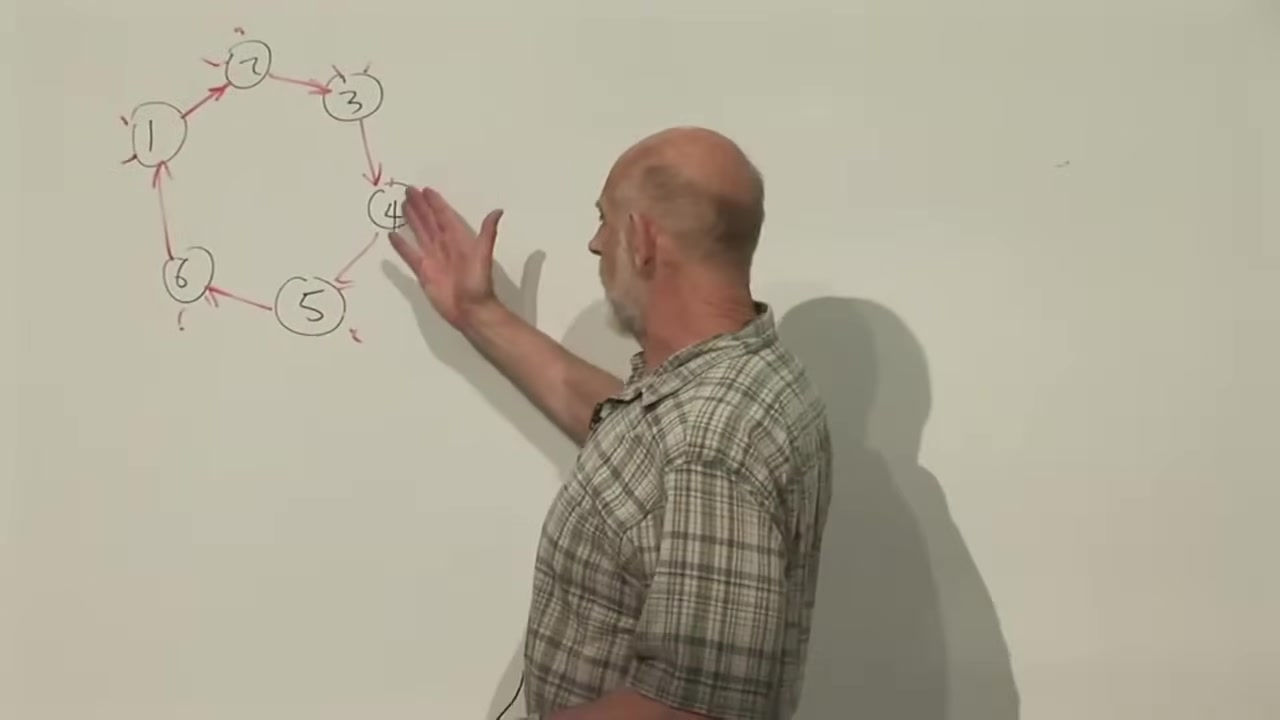
\includegraphics[width=0.86\textwidth]{lecture_01_figure_06.png}
  \caption{単一の6状態サイクル。状態はストロボスコピックな各ステップで次の状態へ移り、6回の更新の後に戻る。}
  \lectureframe{00:12:40}
  \label{fig:six-cycle-board}
\end{figure}

規則は、構造的には異ならないまま、より複雑に見えることがある。例えば、
\begin{equation}
  1\to2\to5\to3\to4\to6\to1
  \label{eq:relabeled-cycle}
\end{equation}
は依然として単一の6サイクルである。頂点を\(1,2,5,3,4,6\)の順にページ上に配置すれば、式~\eqref{eq:six-cycle}と同じ図になる。\(1\)や\(5\)のようなラベルは名前であり、サイクル構造はそれらに依存しない。

真に異なる法則は6つの状態を2つのサイクルに分割する。例えば、
\begin{equation}
  1\to2\to3\to1,
  \qquad
  4\to6\to5\to4.
  \label{eq:two-cycles}
\end{equation}
依然として1つのサイコロと1つの法則があるが、一方のサイクルから始まった軌道は決して他方に到達できない。サイクルに数\(Q\)を付すことができる。
\begin{equation}
  Q=
  \begin{cases}
    0,&\text{on the cycle }\{1,2,3\},\\
    1,&\text{on the cycle }\{4,5,6\}.
  \end{cases}
\end{equation}
状態は各ステップで変化するが、\(Q\)は変化しない。

\begin{definition}
保存量とは、その値が運動法則によって変化しない、状態の関数である。
\end{definition}

同じ考え方により、1つの固定点、1つの2サイクル、1つの3サイクルが可能になる。保存されるラベルは、系がどの軌道に属するかを示す。その軌道内でどの状態にあるかを特定する必要はない。したがって、保存は運動と両立する。保存されるものは必ずしも完全な配置ではなく、可能な配置の間のある区別である。

\begin{figure}[htbp]
  \centering
  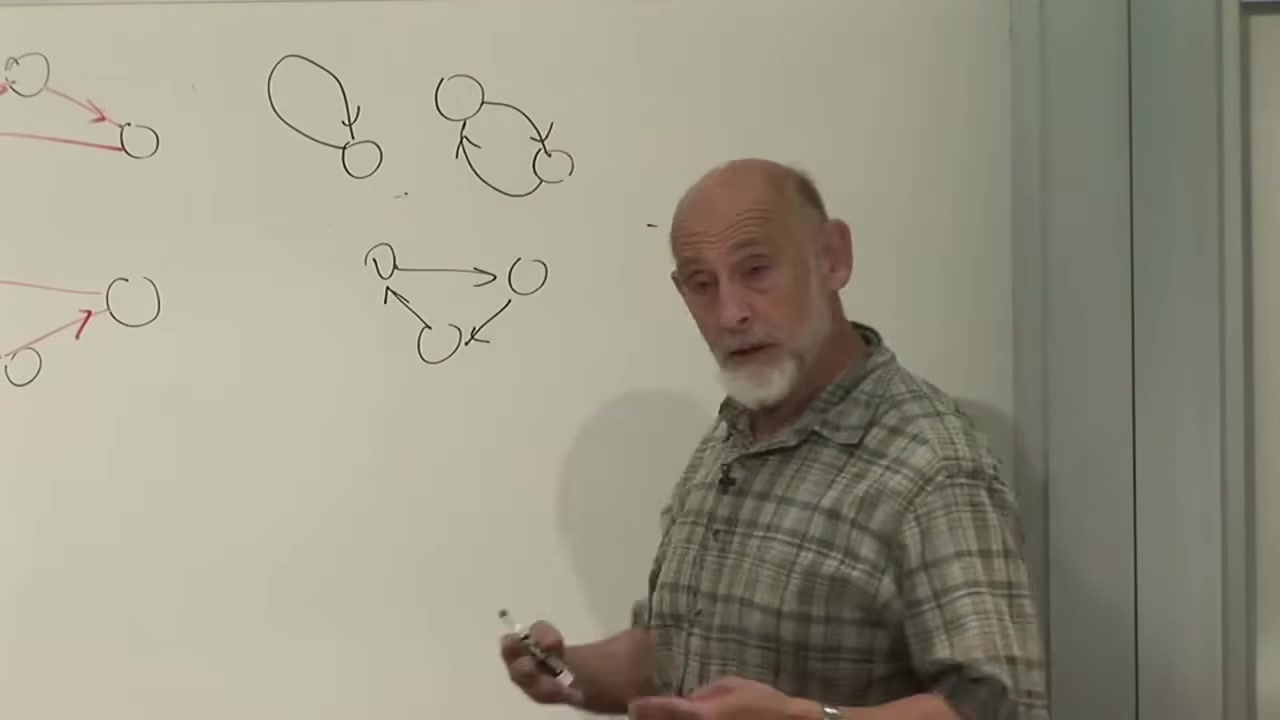
\includegraphics[width=0.86\textwidth]{lecture_01_figure_07.png}
  \caption{盤上のいくつかの連結していないサイクル：固定点、2サイクル、3サイクル。状態がそのサイクルを回っていても、サイクルのラベルは保存される。}
  \lectureframe{00:18:40}
  \label{fig:conserved-cycles-board}
\end{figure}

有限で可逆な系では、すべての軌道はサイクルである。単一のサイクルには、この初等的な種類の非定数な保存ラベルは存在しない。なぜなら、軌道は最終的にすべての状態を訪れるからである。複数のサイクルがあれば、そのようなラベルが可能になる。なぜなら、時間発展は状態を1つの成分から別の成分へ運ぶことが決してないからである。

\section{状態には何を含める必要があるか}

コインの例では1ステップ規則を用いた。次の面は現在の面のみに依存した。聴衆からの質問は、その制限が本質的かどうかを試すものである。

\begin{classroomqa}
\audiencequestion{次の結果が、直ちに見える面だけでなく、おそらく1つまたは複数の以前の結果に依存するような表と裏の列を構成できるだろうか。\lecturetimestamp{00:19:27--00:21:23}}

\lecturerresponse{はい。その場合、\(H\)または\(T\)だけでは完全な状態ではない。1つ前の面が必要なら、状態空間を
\(
  \{HH,HT,TH,TT\}.
\)
に拡大する。各順序対は現在の面と直前の面を記録する。そうすれば、時間発展は再びこの4状態空間上の1ステップ規則として書ける。さらに多くの履歴が必要なら、その情報も含めればよい。}
\end{classroomqa}

この答えは状態の操作的意味を与える。

\begin{definition}
ある時刻における系の状態とは、その未来を予測するために、運動法則とともに必要とされるすべての情報からなる。
\end{definition}

したがって状態は単なる写真ではない。時間発展を確定させる完全なデータの集合こそが状態である。後にニュートン的な粒子を記述するとき、その位置だけでは十分でなく、速度も初期データに属する。記憶をもつコインは、同じ原理の最も単純な版である。

\section{無限の状態空間}

状態が無限個あるからといって、無限個の物体が必要なわけではない。無限直線上の整数サイトに拘束された1つの粒子を考える。その状態は整数
\[
  n\in\mathbb Z.
\]
である。ある法則は各ステップでそれを1サイト右へ動かす：
\begin{equation}
  n(t+1)=n(t)+1.
  \label{eq:lattice-one}
\end{equation}
この軌道は決して閉じないが、未来と過去の両方を通してたどればすべての整数を通過する。その拡張された意味で、それは1つの終わりのないサイクルの役割を果たす。

別の法則は一度に2サイト動かす：
\begin{equation}
  n(t+1)=n(t)+2.
  \label{eq:lattice-two}
\end{equation}
今や偶数のサイトは偶数のサイトのみを通って発展し、奇数のサイトは奇数のサイトのみを通って発展する。パリティは保存される：
\begin{equation}
  \begin{aligned}
    Q_{\rm parity}(n)&=n\bmod 2,\\
    Q_{\rm parity}(n(t+1))&=Q_{\rm parity}(n(t)).
  \end{aligned}
\end{equation}
有限から無限の配置空間への移行は、決して繰り返さない履歴を可能にするが、状態、軌道、保存の意味を変えるものではない。

\section{決定論はまだ可逆性ではない}

ここで、未来を一意に予測するが、古典力学の第二の要件を満たさない規則を提示しよう。三面のコインに表、裏、縁という状態を与え、次を定義する。
\begin{equation}
  H\to T,
  \qquad
  T\to E,
  \qquad
  E\to T.
  \label{eq:nonreversible-map}
\end{equation}
\(H\)から出発すると、履歴は
\[
  H,T,E,T,E,\ldots;
\]
であり、\(T\)または\(E\)のいずれかから出発しても、その後の交替は同様に曖昧さがない。各状態にはちょうど1本の出ていく矢印があるので、この規則は未来に向かって決定論的である。

困難は過去を再構成しようとするときに現れる。現在の状態が\(T\)ならば、その前の状態は\(H\)または\(E\)であった可能性がある。二つの履歴が合流したのである。すべての矢印を逆向きにすれば、欠陥は直ちに明らかになる。\(T\)から、逆向きのグラフは二つの可能な移り先を与える。逆向きの規則は決定論的ではない。

\begin{figure}[htbp]
  \centering
  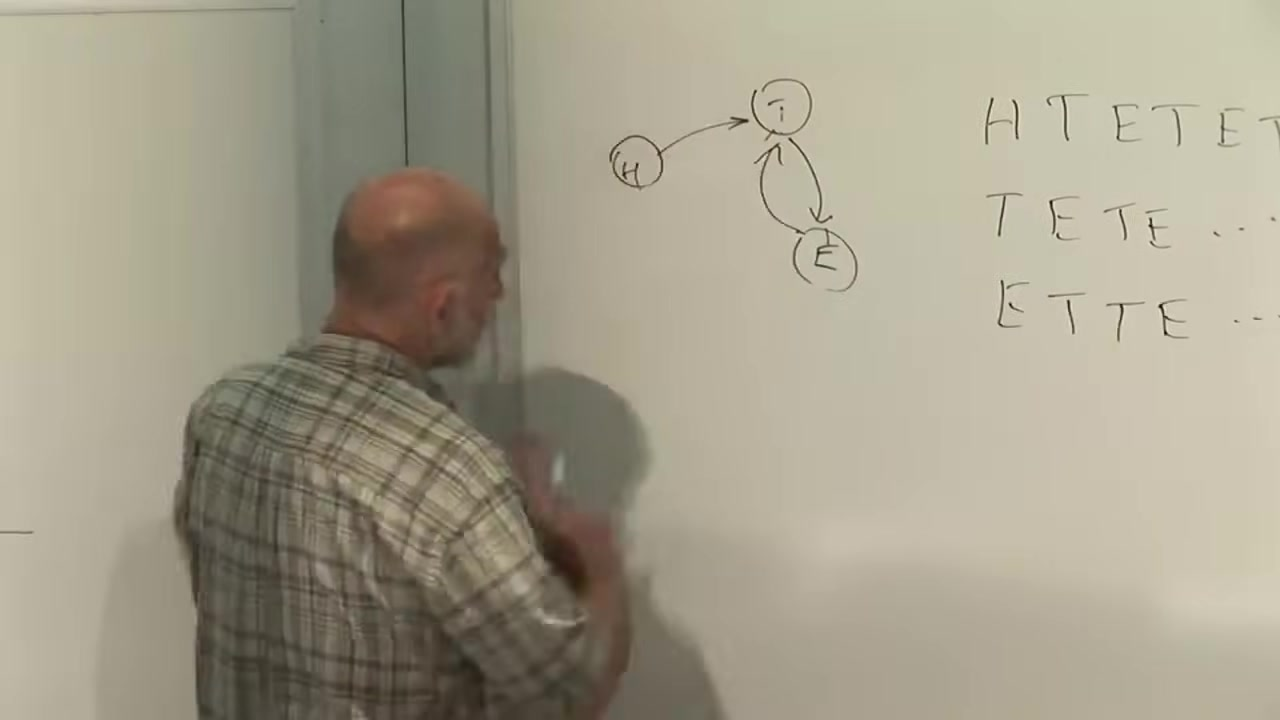
\includegraphics[width=0.86\textwidth]{lecture_01_figure_08.png}
  \caption{非可逆な\(H,T,E\)法則と代表的な履歴。
  \(H\)と\(E\)の両方が\(T\)へと入るので、現在は一意な過去を決定しない。}
  \lectureframe{00:28:50}
  \label{fig:nonreversible-board}
\end{figure}

\begin{definition}
離散的な法則が可逆であるとは、現在の状態が一意な次の状態と一意な前の状態の両方を決定するときをいう。状態グラフでは、各状態がちょうど1本の出ていく矢印とちょうど1本の入ってくる矢印をもたなければならない。
\end{definition}

有限な状態空間に対して、可逆な更新は状態の置換である。それは状態間の区別を生成も破壊もしない。ただそれらを並べ替えるだけである。これが、そのグラフがサイクルに分解される理由である。式~\eqref{eq:nonreversible-map}の写像は関数であるが、一対一の関数ではないため、逆写像をもたない。

\begin{classroomqa}
\audiencequestion{この種の規則が、状態が粒子の確率を表すものであるならば許されるだろうか。\lecturetimestamp{00:29:46--00:31:17}}

\lecturerresponse{それは別の枠組みであろう。ここで定式化されている基礎的な古典力学は、確率的な更新規則ではなく決定論的法則を用いる。そのような規則を考案して研究することはもちろんできるが、この意味での古典力学的法則ではない。量子力学は同じ意味では決定論的でないが、それでも可逆な発展の類似物をもつ。それには後の議論が必要である。古典統計力学も確率を用いるが、それは基礎にある力学的法則から出発し、その初期データに関する不完全な知識を表す。}
\end{classroomqa}

この区別は重要である。正確な古典的状態を知らないために用いられる確率分布は、非決定論的な運動法則ではない。それは、微視的発展が依然として決定論的かつ可逆的であるとみなされる系についての我々の情報を記述するものである。

\section{厳密な法則と不完全な知識}

予測には二つの要素が必要である。
\begin{enumerate}
  \item 運動法則。
  \item 初期状態。
\end{enumerate}
厳密な法則も、初期条件が近似的にしか知られていないときには、厳密な予報を生み出さない。コインの場合、机を見て面を完全に知ることを想像するのは容易である。実際の力学的変数は連続的である。位置と速度は任意の実数値をとり得て、いかなる測定も無限桁の小数を与えない。

真の初期状態が可能な状態の小さな領域内にあるとしよう。ある力学の下ではその領域は長い間小さいままだが、別の力学の下では近くの初期状態が急速に離れていく。カオス系では、小さな初期の不確かさが最終的に大きな差へと成長する。大気はよく知られた例である。より良い測定は有用な予報を延ばし得るが、どんな固定された測定精度に対しても、予報が信頼できなくなる十分に遠い時刻が存在する。

この実際上の制限は方程式に曖昧さを持ち込まない。初期条件が正確に知られていれば、古典的な可逆法則は未来と過去の両方を決定するであろう。有限の精度のもとでは、代わりに定量的な問いは次である。指定された長さの時間に対する予測を行うために、初期状態はどれほど正確に知られなければならないか。

図による判定は今や簡潔な結論をもつ。各状態において1本の入ってくる矢印と1本の出ていく矢印で表される法則は、決定論的かつ可逆である。粒子に対応する主張はより初等的でなくなるが、同じ古典的構造を表している。

\section{抽象状態から空間内の点へ}

次に、硬貨やサイコロから質点へと話を移す。質点は1次元、3次元、5次元、あるいはその他の任意の次元を運動しうるが、通常の空間が直ちに具体例を与える。点を定量的に記述するには、次を選ぶ：
\begin{itemize}
  \item 原点；
  \item 互いに垂直な3本の軸；
  \item それらの軸の向き；
  \item 長さの単位。
\end{itemize}
原点は慣習的なものである。原点はパロアルトに置いてもどこに置いてもよく、物理的な結論はその選択に依存すべきではない。軸には\(x,y,z\)、または\(x_1,x_2,x_3\)とラベルを付けてもよい。\(x\)方向と\(y\)方向を固定した後、\(z\)軸は垂直な2方向のいずれかを向きうる。我々は右手系の慣習を選ぶ：右手の親指を\(x\)に沿わせ、人差し指を\(y\)に沿わせると、中指は\(z\)に沿って指し示す。

軸に沿った等間隔の目盛りには、メートル、フィート、インチ、光年などの単位が必要である。これらの慣習をひとたび固定すれば、すべての点は3つの数
\begin{equation}
  (x,y,z).
\end{equation}
によってラベル付けされる。原点から3本の軸に沿った変位によってその点に到達できる。多数の質点からなる系では、各質点に対してそのような三つ組が1つ必要である。

\begin{figure}[htbp]
  \centering
  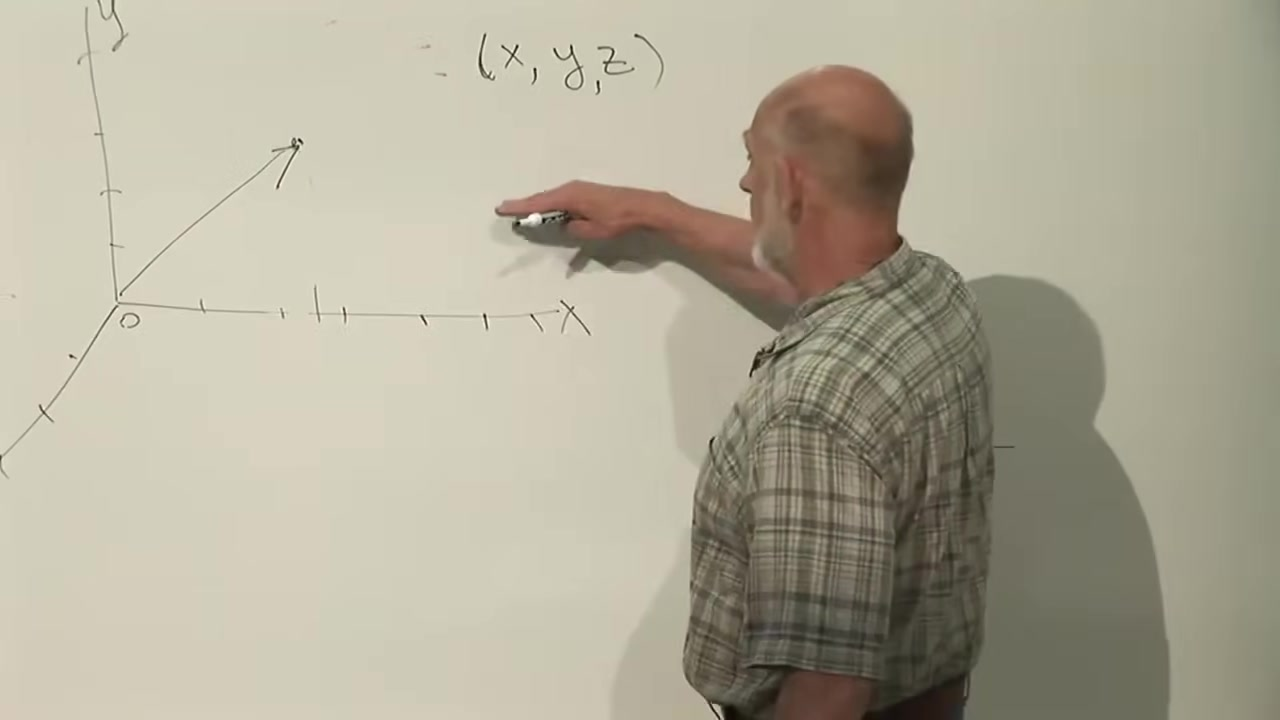
\includegraphics[width=0.86\textwidth]{lecture_01_figure_09.png}
  \caption{デカルト軸と点の3つの座標。図は座標の慣習を固定する；点そのものは、原点や軸をどこに置くよう選ぶかには依存しない。}
  \lectureframe{00:43:00}
  \label{fig:coordinates-board}
\end{figure}

\section{ベクトルとその成分}

ベクトルとは大きさと向きをもつ対象である。原点から点への変位はベクトルであるが、ベクトルは速度、加速度、電場、その他多くの量も記述する。ベクトルは\(\mathbf v\)のように太字で書き、その大きさを\(\lvert\mathbf v\rvert\)と書くことにする。大きさは非負であり、零ベクトルのみでゼロになる。

幾何学的には、ベクトルは自由な矢印である。長さや向きを変えずに矢印を平行移動してもベクトルは変わらない。特定の応用では、与えられた位置における電場を指定するときのように、ベクトルを点に付随させることができるが、付随は追加の情報であり、抽象的なベクトルそのものの一部ではない。

デカルト軸に対して、ベクトルは成分
\begin{equation}
  \mathbf v=(v_x,v_y,v_z).
\end{equation}
をもつ。成分は通常の符号付きの数であり、軸への射影によって得られる。それらは大きさと向きの両方を符号化する。3次元のピタゴラスの定理により
\begin{equation}
  \lvert\mathbf v\rvert^2
  =v_x^2+v_y^2+v_z^2,
  \qquad
  \lvert\mathbf v\rvert
  =\sqrt{v_x^2+v_y^2+v_z^2}.
  \label{eq:vector-magnitude}
\end{equation}
が成り立つ。成分の比が向きを定める。負の成分は、ベクトルがその軸の負の方向に部分的に沿って指していることを意味する。

\subsection{スカラー倍と加法}

実数による乗法はベクトルの長さを変え、その数が負であれば向きを逆にする。\(c>0\)に対して、\(c\mathbf A\)は\(\mathbf A\)の向きを向き、大きさ
\(c\lvert\mathbf A\rvert\)
をもつ。特に、\(-\mathbf A\)は\(\mathbf A\)と同じ長さをもち、逆向きを向く。

ベクトルの加法には3つの等価な描像がある。第一に、\(\mathbf B\)の尾を\(\mathbf A\)の頭に置く；\(\mathbf A\)の尾から\(\mathbf B\)の頭への矢印が\(\mathbf A+\mathbf B\)である。第二に、両方の尾を一緒に置いて平行四辺形を完成させる；その対角線が和である。この形は可換性を可視化する：
\begin{equation}
  \mathbf A+\mathbf B=\mathbf B+\mathbf A.
\end{equation}
第三に、対応する成分を加える：
\begin{equation}
  C_i=A_i+B_i,
  \qquad i=x,y,z,
  \label{eq:component-addition}
\end{equation}
ここで\(\mathbf C=\mathbf A+\mathbf B\)である。これらの規則は\(a\mathbf A+b\mathbf B\)のような任意の線形結合も定義する。

\begin{figure}[htbp]
  \centering
  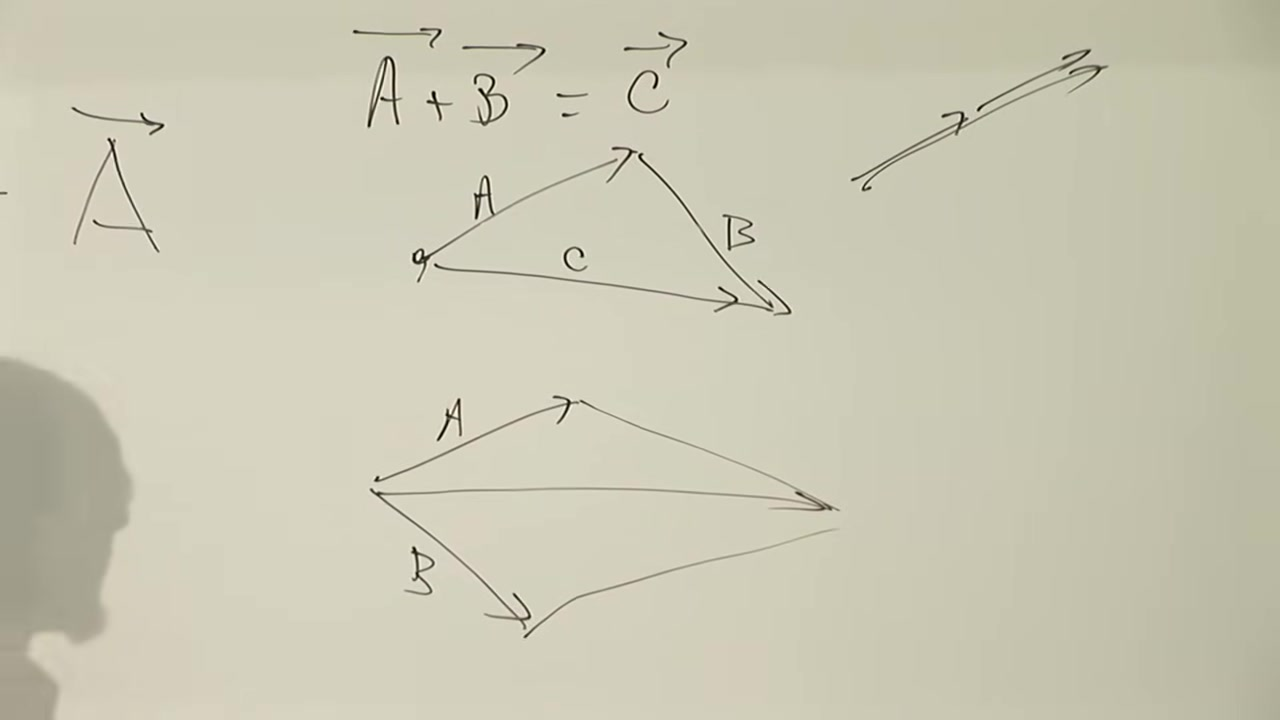
\includegraphics[width=0.86\textwidth]{lecture_01_figure_10.png}
  \caption{ベクトル加法のための三角形と平行四辺形の作図。どちらも同じベクトル\(\mathbf A+\mathbf B\)を与える。}
  \lectureframe{00:53:00}
  \label{fig:vector-addition-board}
\end{figure}

あるベクトルを別のベクトルで割るという一般的な演算は存在しない。しかし、2つの標準的なベクトル積がある。外積は後の講義に残す。ここでは内積が必要である。

\subsection{内積}

\(\mathbf A\)を\(\mathbf B\)の定める軸に射影する。ベクトル間の角を\(\theta\)とすると、\(\mathbf B\)に沿った\(\mathbf A\)の符号付き成分は\(\lvert\mathbf A\rvert\cos\theta\)である。この射影に\(\lvert\mathbf B\rvert\)を掛けると
\begin{equation}
  \mathbf A\cdot\mathbf B
  =\lvert\mathbf A\rvert\,\lvert\mathbf B\rvert\cos\theta.
  \label{eq:dot-geometric}
\end{equation}
が定義される。結果はスカラーであり、別のベクトルではない。式~\eqref{eq:dot-geometric}は\(\mathbf A\)と\(\mathbf B\)に関して対称であるから、
\(\mathbf A\cdot\mathbf B=\mathbf B\cdot\mathbf A\)
である。

\begin{figure}[htbp]
  \centering
  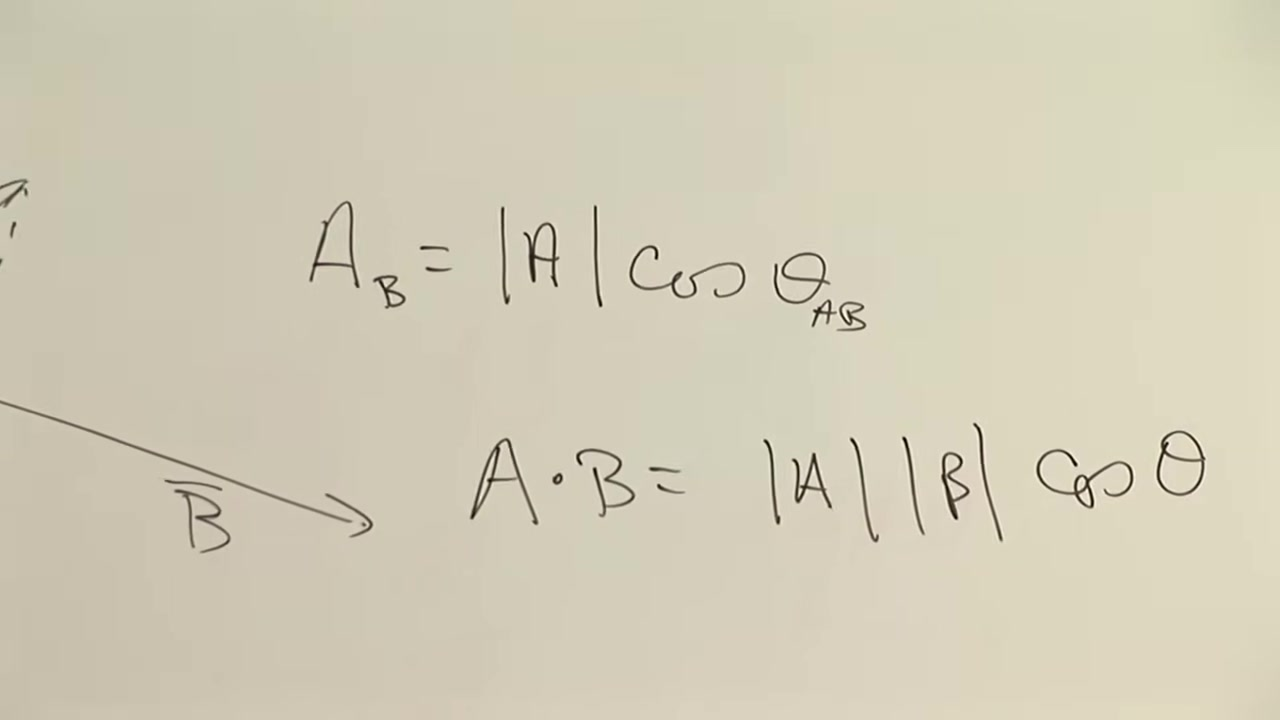
\includegraphics[width=0.86\textwidth]{lecture_01_figure_11.png}
  \caption{射影による内積の黒板での構成。組版された形は
  \(\mathbf A\cdot\mathbf B=AB\cos\theta\)
である。}
  \lectureframe{00:58:30}
  \label{fig:dot-product-board}
\end{figure}

符号は幾何学的情報を担う。内積は鋭角に対して正、鈍角に対して負、垂直なベクトルに対してゼロである。したがって、非零ベクトルに対して
\begin{equation}
  \mathbf A\perp\mathbf B
  \quad\Longleftrightarrow\quad
  \mathbf A\cdot\mathbf B=0
\end{equation}
が成り立つ。

成分で表すと，
\begin{equation}
  \mathbf A\cdot\mathbf B
  =A_xB_x+A_yB_y+A_zB_z.
  \label{eq:dot-components}
\end{equation}
この式により計算は即座にできる。特に，
\begin{equation}
  \mathbf A\cdot\mathbf A
  =A_x^2+A_y^2+A_z^2
  =\lvert\mathbf A\rvert^2.
  \label{eq:self-dot}
\end{equation}
二つのベクトルの成分が与えられれば，式~\eqref{eq:dot-geometric}と式\eqref{eq:dot-components}によりそれらのなす角が定まる：
\begin{equation}
  \cos\theta
  =\frac{\mathbf A\cdot\mathbf B}
  {\lvert\mathbf A\rvert\,\lvert\mathbf B\rvert}.
\end{equation}

余弦定理は同じ代数から導かれる。\(\mathbf A\)と\(\mathbf B\)が共通の頂点から三角形の他の二つの頂点へ向かうとする。第三の辺は
\(\mathbf C=\mathbf A-\mathbf B\)であり，\(\mathbf A+\mathbf B\)ではない。したがって
\begin{align}
  C^2
  &=(\mathbf A-\mathbf B)\cdot(\mathbf A-\mathbf B)\notag\\
  &=A^2+B^2-2\mathbf A\cdot\mathbf B\notag\\
  &=A^2+B^2-2AB\cos\theta.
  \label{eq:law-of-cosines}
\end{align}

\begin{figure}[htbp]
  \centering
  \includegraphics[width=0.86\textwidth]{lecture_01_figure_04.png}
  \caption{余弦定理に用いる三角形。板書の訂正は閉じる辺を
  \(\mathbf C=\mathbf A-\mathbf B\)と同定し，式~\eqref{eq:law-of-cosines}を導く。}
  \lectureframe{01:04:29}
  \label{fig:law-cosines-board}
\end{figure}

\section{位置，速度，加速度}

原点を選び，\(\mathbf r\)を原点から質点への位置ベクトルとする。その成分はデカルト座標である：
\begin{equation}
  \mathbf r=(x,y,z),
  \qquad
  \lvert\mathbf r\rvert=\sqrt{x^2+y^2+z^2}.
\end{equation}
原点を変えれば\(\mathbf r\)が変わるが，この問題は後回しにする。いったん原点を固定すれば，運動は時間に依存する位置
\begin{equation}
  \mathbf r(t)=\bigl(x(t),y(t),z(t)\bigr).
\end{equation}
によって記述される。したがって軌道は三つの時間の関数によって符号化される。

速度は位置の時間微分である：
\begin{equation}
  \mathbf v(t)=\frac{d\mathbf r}{dt}
  =\dot{\mathbf r}(t),
  \qquad
  v_i=\frac{dx_i}{dt}=\dot x_i.
  \label{eq:velocity}
\end{equation}
ドットは常に時間に関する微分を表す。大きさ\(\lvert\mathbf v\rvert\)が速さである。位置と速度は一般に独立な方向をもつ：ある位置にある質点は，問題が許す任意の方向に運動していてよい。

加速度は速度の変化率であり，したがって位置の二階時間微分である：
\begin{equation}
  \mathbf a(t)=\frac{d\mathbf v}{dt}
  =\dot{\mathbf v}(t)
  =\frac{d^2\mathbf r}{dt^2}
  =\ddot{\mathbf r}(t),
  \qquad
  a_i=\ddot x_i.
  \label{eq:acceleration}
\end{equation}
加速度もまたベクトルである。正の\(x\)方向に運動する質点が速くなるとき，\(a_x>0\)である。遅くなるとき，\(a_x<0\)である。しばしば減速と呼ばれるものは，現在の速度と逆向きの加速度にほかならない。より一般には，大きさが一定のままであっても，方向を変えることによって速度は変化しうる。

\begin{figure}[htbp]
  \centering
  \includegraphics[width=0.86\textwidth]{lecture_01_figure_05.png}
  \caption{位置成分の時間微分として書かれた速度成分。簡潔なベクトル表記では，
  \(\mathbf v=d\mathbf r/dt\)。}
  \lectureframe{01:14:24}
  \label{fig:velocity-board}
\end{figure}

\subsection{直線上の等加速度運動}

一次元運動について，
\begin{equation}
  x(t)=a+bt+ct^2.
  \label{eq:quadratic-motion}
\end{equation}
と書く。\(t=0\)において，質点は\(x=a\)にある。一階微分し，次に二階微分すると
\begin{align}
  v(t)=\dot x(t)&=b+2ct,\label{eq:line-velocity}\\
  a(t)=\ddot x(t)&=2c.\label{eq:line-acceleration}
\end{align}
が得られる。したがって\(b\)は初速度であり，\(2c\)は一定の加速度である。\(c>0\)ならば速度は線形に増加し，\(c<0\)ならば線形に減少する。この二次式で表される位置の法則は，一定の加速度のもとでの運動，たとえば地球表面近くでの落体の理想化された運動がとる形である。

\section{等速円運動}

最後の例として，質点が\(x\)-\(y\)平面内の単位円上を運動するとする。質点は\(t=0\)において正の\(x\)軸上から出発し，その角度座標は一様に増加する：
\begin{equation}
  \theta(t)=\omega t.
\end{equation}
定数\(\omega\)は角振動数である。一回転は角度の増加\(2\pi\)に対応するので，周期は
\begin{equation}
  T=\frac{2\pi}{\omega}.
  \label{eq:circular-period}
\end{equation}
角度は\(2\pi\)を超えて増加してもよい；連続的に記録された角度はリセットされないが，位置は繰り返す。

単位円上では，
\begin{equation}
  \mathbf r(t)
  =\bigl(\cos\omega t,\,\sin\omega t\bigr).
  \label{eq:circular-position}
\end{equation}
微分すると
\begin{equation}
  \mathbf v(t)
  =\omega\bigl(-\sin\omega t,\,\cos\omega t\bigr).
  \label{eq:circular-velocity}
\end{equation}
速度は円に接する。図に頼ることなく，半径に対する垂直性を証明できる：
\begin{align}
  \mathbf r\cdot\mathbf v
  &=\cos\omega t\,(-\omega\sin\omega t)
    +\sin\omega t\,(\omega\cos\omega t)\notag\\
  &=0.
  \label{eq:r-dot-v}
\end{align}

\begin{figure}[htbp]
  \centering
  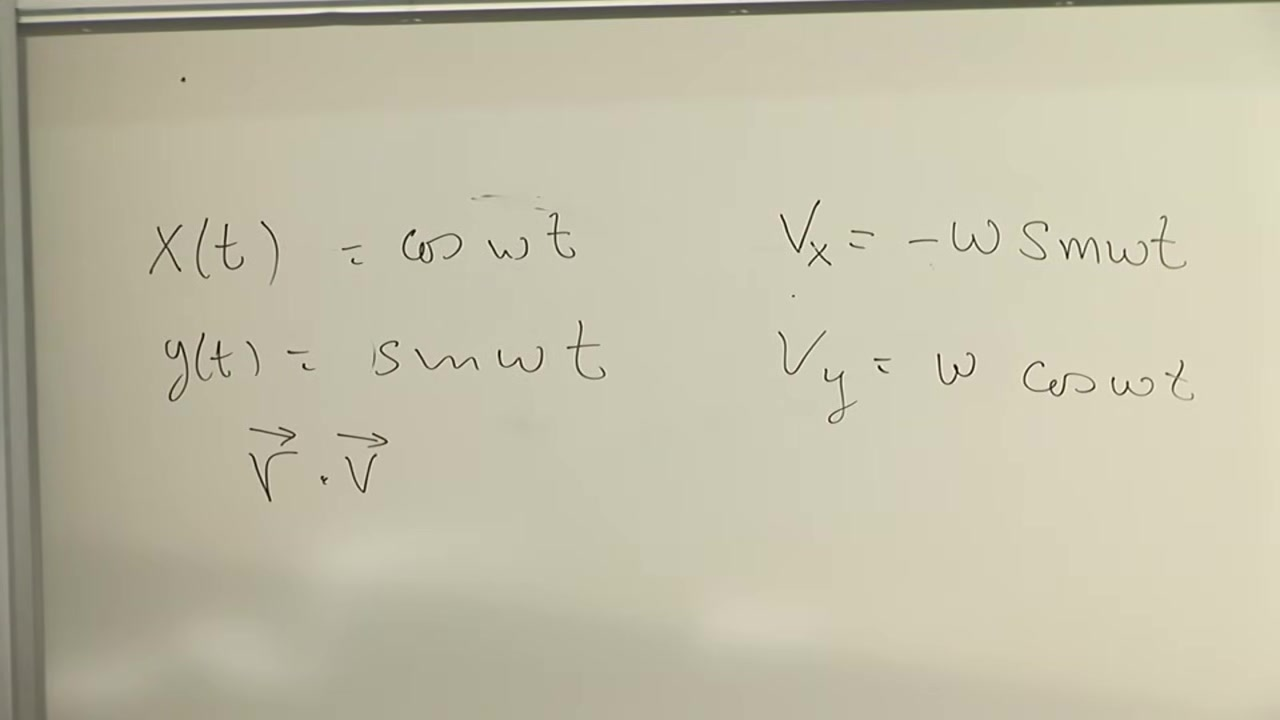
\includegraphics[width=0.86\textwidth]{lecture_01_figure_12.png}
  \caption{単位円上の運動に対する位置と速度の成分。
  \(\mathbf r\cdot\mathbf v\)における相殺は，速度が
  円に接することを検証する。}
  \lectureframe{01:24:30}
  \label{fig:circular-velocity-board}
\end{figure}

もう一度微分すると，
\begin{equation}
  \mathbf a(t)
  =-\omega^2
  \bigl(\cos\omega t,\,\sin\omega t\bigr)
  =-\omega^2\mathbf r(t).
  \label{eq:centripetal-acceleration}
\end{equation}
加速度は半径に平行であるが，反対向きに，すなわち中心へ向かって指す。これが向心加速度である。\footnote{用語に関する注意：講義ではこの時点で``遠心力''という語が現れるが，式と付随する説明は，中心へ向かう標準的な向心加速度を同定している。}

\begin{figure}[H]
  \centering
  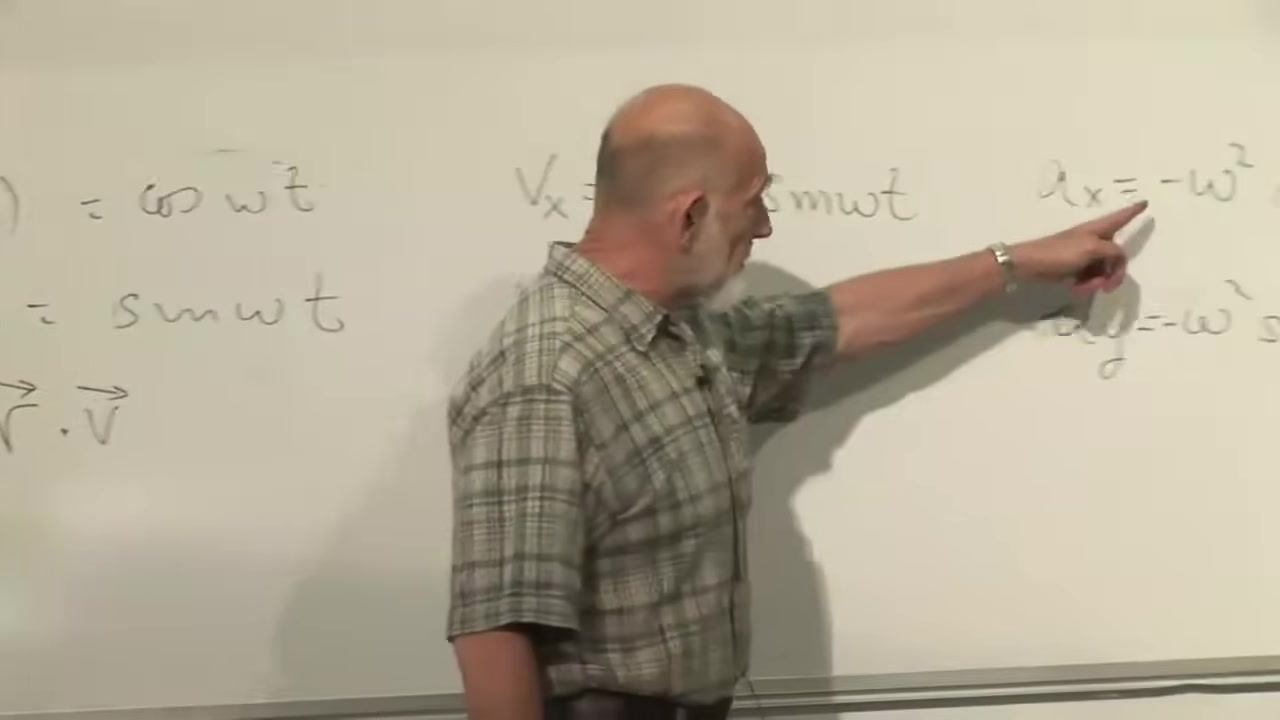
\includegraphics[width=0.86\textwidth]{lecture_01_figure_13.png}
  \caption{円運動の加速度の成分計算。各成分は対応する位置成分の
  \(-\omega^2\)倍であるので，
  \(\mathbf a=-\omega^2\mathbf r\)。}
  \lectureframe{01:26:30}
  \label{fig:circular-acceleration-board}
\end{figure}

半径が一であるので，
\begin{equation}
  \lvert\mathbf r\rvert=1,
  \qquad
  \lvert\mathbf v\rvert=\omega,
  \qquad
  \lvert\mathbf a\rvert=\omega^2.
\end{equation}
\(\omega\)を増加させると，速さは線形に増加し，必要な内向きの加速度は二次的に増加する。半径\(R\)の円に対しては，同じ計算により\(v=\omega R\)および
\(\lvert\mathbf a\rvert=\omega^2R=v^2/R\)が得られるであろう；講義では最初の計算を煩雑にしないために\(R=1\)を用いている。

これで、質点力学に必要な初等的な言語が揃った。すなわち、状態と初期データ、可逆な時間発展、座標、ベクトル、そして速度と加速度を定義する導関数である。次の課題は、どの初期データが質点を指定するのかを正確に定め、それらのデータをある瞬間から次の瞬間へと運ぶ法則を見出すことである。